% !TEX encoding = UTF-8 Unicode
\documentclass{beamer}

\usepackage{beamerthemesplit} 
\usepackage[utf8]{inputenc}


\title{Der Kampf für die Informationsfreiheit ist ein sozialer}
\author{Daniel Schweighöfer}
\date{\today}

\begin{document}

\frame{\titlepage}

\section[Einführung]{}

\frame
{
  \frametitle{Der Typ da vorne}

  \begin{itemize}
  \item acid (leider noch @acid23 )
  \item Daniel Schweighöfer
  \item redet, denkt und schreibt. Arbeitet als Webentwickler oder Administrator
  \item Spackeria, Feminismus, Unziivilisation...
  \item http://netsteward.net
  \end{itemize}
}

\frame{\tableofcontents}

\section{Informationsfreiheit im und durch das Netz}
\subsection{Echt ne gute Sache...}

\frame
{
  \frametitle{Informationsfreiheit im und durch das Netz}
  Echt ne gute Sache...
}

\frame
{
  \frametitle{denn sie...}

  \begin{itemize}[<+->]
  \item fördert die Entwicklung von Politik und Kultur
  \item lässt Menschen näher zusammen wachsen
  \item verstärkt soziale Phänomene
  \end{itemize}
}

\subsubsection{Beispiele für positive soziale Phänomene}

\frame
{
  \frametitle{Graswurzel-Bewegungen}
   \begin{figure}[p] %  figure placement: here, top, bottom, or page
     \centering
     
\includegraphics[width=2.5in]{telecomix.png} 
  \end{figure}
}
\frame
{
  \frametitle{Hypes}
    \begin{figure}[p] %  figure placement: here, top, bottom, or page
     \centering
     
\includegraphics[width=3in]{RiotPwny.jpg} 
  \end{figure}
}

\subsection{... aber auch mit großem Haken}

\frame{
  \frametitle{Informationsfreiheit im und durch das Netz}
  ... aber auch mit großem Haken
}
\frame
{
  \frametitle{denn sie...}

  \begin{itemize}[<+->]
  \item fördert das Aufzeigen von kulturell-/sozialen Unterschieden
  \item erleichtern soziale Isolation/Seperation
  \item verstärkt soziale Phänomene
  \end{itemize}
}

\subsubsection{Beispiele für negative soziale Phänomene}
\frame
{
  \frametitle{Shitstorms}
  \begin{figure}[p] %  figure placement: here, top, bottom, or page
     \centering
     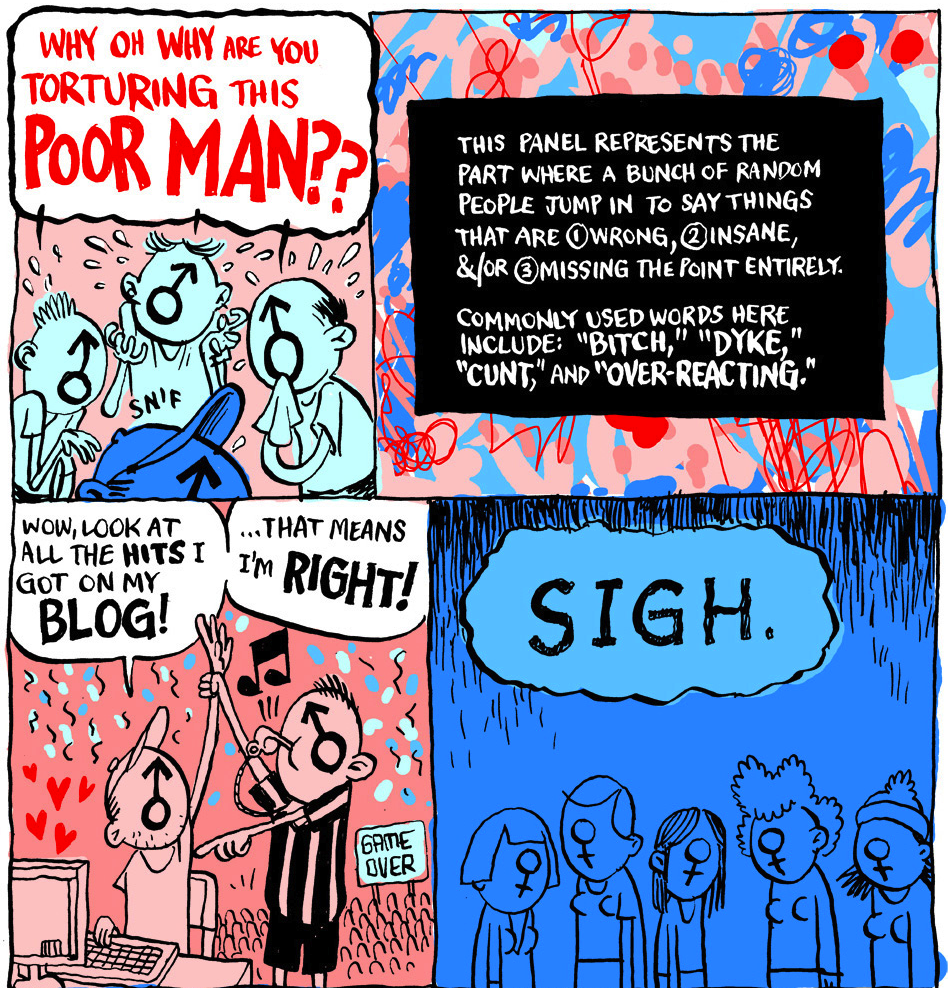
\includegraphics[width=2in]{shitstorm.png} 
  \end{figure}
}
\frame
{
  \frametitle{Raids}
  \begin{figure}[p] %  figure placement: here, top, bottom, or page
     \centering
     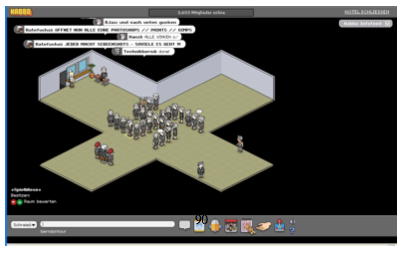
\includegraphics[width=4in]{raid.png} 
  \end{figure}
}

\section{It's all about privileges!}
\subsection{Das Märchen vom Default-Menschen}

\frame{
  \frametitle{It's all about privileges!}
  Das Märchen vom Default-Menschen
}
\frame
{
  \frametitle{Sei...}
  
  \begin{itemize}[<+->]
  \item weiß,
  \item männlich,
  \item sowie nicht zu alt
  \end{itemize}
  
  \begin{block}<4->{Und die Welt gehört dir!}
  \end{block}
}
\frame
{
  \frametitle{Exkurs: Konzept der einen Wahrheit}
  
  Mensch geht davon aus, dass es eine allgemeingültige Wahrheit gäbe.
  Davon abweichende Ansichten werden
  \begin{itemize}
    \item grundsätzlich in Frage gestellt
    \item als weniger gültig betrachtet.
  \end{itemize}
}
\subsection{Privilegien}

\frame
{
  \frametitle{It's all about privileges!}
  Privilegien
}
\frame
{
  \frametitle{Wer?}
  
  Menschen, denen die arbiträren "defaults" zugesprochen werden, sind privilegiert.
}
\frame
{
  \frametitle{Wie?}
  
  Priviligiert sein heißt
  \begin{itemize}[<+->]
  \item von anderen bevorzugt bzw. nicht besonders behandelt werden
  \item sich sozialem Rückhaltes sicher sein
  \end{itemize}
}
\frame
{ 
  \frametitle{Was ist daran schlecht?}
  
  Menschen in der Informationsfreiheit brauchen
  \begin{itemize}[<+->]
  \item soziale Sicherheit
  \item (maximal) erweiterte Schutzräume 
  \item freie Wahl von Identitäten
  \end{itemize}
  
  \begin{theorem}<4->
    Eine von Privilegien geprägte Gesellschaft wie die unsere jetzige droht die positiven Effekte der Informationsfreiheit zu negieren! 
  \end{theorem}
}
\subsection{Mechanismen zur Etablierung und Stärkung von Privilegien}

\frame
{
  \frametitle{It's all about privileges!}
  Mechanismen zur Etablierung und Stärkung von Privilegien
}
\frame
{
  \frametitle{Ein bunter Strauß Begriffe aus den Sozialwissenschaften}
  
  \begin{itemize}[<+->]
  \item Exklusion
  \item Fremdmarkierung
  \item Normen
  \item Geld
  \item systematischer Matcherhalt
  \end{itemize}
}
\section{Aktionsvektoren}
\subsection{-ismen ftw!}

\frame
{
  \frametitle{Aktionsvektoren}
  -ismen ftw!
}
\frame
{
  \frametitle{Pluralismus}
  
  Die Diversität der Lebens- und Denkweisen muss gefördert werden!
}
\frame
{
  \frametitle{Feminismus}
  
  Eine wichtige Bewegung die den meisten kaum vertraut ist. Das sollten wir ändern, um
  \begin{itemize}[<+->]
  \item voneinander zu lernen und
  \item einen eigenen, offeneren Feminismus zu prägen.
  \end{itemize}

}
\frame
{
  \frametitle{Anarchiismus}
  
  Viele bekannte Probleme aber auch verstaubte Geister.
  \begin{itemize}[<+->]
  \item Menschenbildproblematik
  \item Diskussionskultur
  \end{itemize}

}
\frame
{
  \frametitle{Erklärbär(-ismus)}
  
  \begin{itemize}[<+->]
  \item unheimlich wichtig
  \item unheimlich anstrengend
  \item unheimlich belohnend
  \end{itemize}
  
}
\subsection{Die große Frage}

\frame
{
  \frametitle{Aktionsvektoren}
  Die große Frage
}
\frame
{
  \frametitle{Wie auf einen Angriff reagieren?}
  
  \begin{itemize}[<+->]
  \item wehren => anpassen => nicht weiter entwickelt
  \item fliehen => aufgeben => aus der Evolution verabschieden
  \item reden? energisch friedlich bleiben? Auf den großen Crash warten?
  \end{itemize}

}
\frame
{
  \frametitle{Danke!}
  
  \begin{itemize}
  \item Fragen?
  \item Kritik?
  \item Anregungen?
  \item Code? https://github.com/acid/Spack0-Talk
  \end{itemize}

}
\end{document}
